\documentclass[conference]{IEEEtran}
\IEEEoverridecommandlockouts
% The preceding line is only needed to identify funding in the first footnote. If that is unneeded, please comment it out.
\usepackage[utf8]{inputenc}
\usepackage[croatian]{babel}
\usepackage{cite}
\usepackage{array}
\usepackage{amsmath,amssymb,amsfonts}
\usepackage{algorithmic}
\usepackage{graphicx}
\usepackage{textcomp}
\usepackage{xcolor}
\usepackage{times}
\usepackage{fancyhdr}
\usepackage[ruled,vlined]{algorithm2e}
\include{pythonlisting}
\usepackage[croatian]{babel}
\def\BibTeX{{\rm B\kern-.05em{\sc i\kern-.025em b}\kern-.08em
    T\kern-.1667em\lower.7ex\hbox{E}\kern-.125emX}}

\renewcommand\IEEEkeywordsname{Ključni pojmovi}
\DeclareMathOperator{\taninv}{tan^{-1}}

\begin{document}

\title{Segmentacija slike - detekcija ivica}

\author{\IEEEauthorblockN{Muaz Kasumovi\'c}
\IEEEauthorblockA{\textit{Odsjek za Teorijsku kompjutersku nauku} \\
\textit{Prirodno-matemati\v{c}ki fakultet Sarajevo}\\
Sarajevo, BIH \\
muazkasumovic@gmail.com}
\
}

\maketitle

\begin{abstract}
Detekcija ivica je vrsta tehnika segmentacije slike koja određuje prisustvo ivica na slici i ocrtava ih na odgovarajući način. Glavna svrha otkrivanja ivica je da se pojednostave podaci o slici kako bi se smanjila količina podataka za obradu. Ivica se definira kao značajna lokalna promjena intenziteta slike. Ivice se najčešće pojavljuju na granici između dva različita područja na slici. U ovom radu su predstavljene metode za segmentaciju ivica slike. Obrađene su  četiri metode za detekciju ivica: metoda koja koristi Sobelov operator, Prewittov operator, Laplasova metoda i Canny metoda. Ove metode su implementirane u programskom jeziku Matlab. Na kraju rada je data usporedba ovih metoda međusobno kao i usporedba sa Matlab-ovim ugrađenim funkcijama te vremena izvršavanja pomenutih funkcija.
\end{abstract}

\begin{IEEEkeywords}
detekcija ivica, Sobelov operator, Prewittov operator, Laplasova metda, Canny metoda.
\end{IEEEkeywords}

\section{Uvod}
Intuitivno ivica se može smatrati kao skup povezanih piksela koji leže na granici između dvije oblasti na slici. Da bismo definisali ivicu moramo imati način da izmjerimo tranziciju u nivou sive boje.   Idealna ivica se može smatrati kao skup povezanih piksela od kojih je svaki lociran na ortogonalnom step prelazu nivoa sive boje kao što je prikazano na slici 1. U praksi zbog optičkih nesavršenosti, nesavršenosti uzorkovanja i drugih nesavršenosti sistema za akviziciju slike imamo da su ivice zamagljene (engl. blurred) sa stepenom zamagljenja određenim faktorima kao što su kvalitet sistema za akviziciju slike, brzina uzorkovanja i osvjetljenje u kojem je slika akvizirana. Posljedica ovog svega je da ivice vjerodostojnije možemo modelirati kao rampu (slika 1.) pri čemu je koeficijent nagiba obrnuto proporcionalan
stepenu zamagljenja slike.


\begin{figure}[htbp]
\centerline{\includegraphics[scale =0.3]{idealnaivica.jpg}
   \hspace{1.5cm}
\includegraphics[scale =0.3]{realnaivica.jpg}
}
\caption{Model idealne i realne ivice}
\label{fig}
\end{figure}

U ovom modelu ivice više nisu tanke (debljine 1 piksel) već u ivicu se uključuju svi pikseli koji pripadaju rampi. Debljina ivice je određena dužinom rampe koja je određena koeficijentom nagiba.\cite{b1} Pregled metoda za detekciju ivica se može pogledati u \cite{b2}.


\section{Detekcija ivica pomoću izvoda}
Na slici 2 je prikazan horizontalni profil nivoa sive boje ivice između dvije oblasti.Na slici su također prikazani prvi i  drugi izvod ovog profila nivoa sive. Prvi izvod je pozitivan u tačkama prelaska na i sa rampe i u tačkama na rampi u kojima je također i konstantan dok je nula u tačkama gdje je nivo sive konstantan. Drugi izvod je pozitivan u prelazu koji pridružem tamnoj strani dok je negativan u prelazu pridruženom svijetloj ivici te nula  duž rampe i u tačkama konstantnog nivoa sive.    
\begin{figure}[htbp]
\centerline{\includegraphics[scale =0.5]{izvod.jpg}
}
\caption{Prva kolona: slika i profil nivoa sive, Druga kolona: prvi izvod slike i profil nivoa sive, Treća kolona: drugi izvod slike i profil nivoa sive}
\label{fig}
\end{figure}
Na osnovu ovih opservacija možemo zaključit da se intenzitet prvog izvoda može iskoristit za detekciju da li tačka pripada ivici odnosno da li tačka pripada rampi. Slično, znak drugog izvoda možemo iskoristiti da odredimo da li se piksel nalazi na tamnoj ili svijetloj strani ivice. Možemo primjetiti još dvije osobine drugog izvoda: za svaku ivicu na slici  dobijamo dvije vrijednosti; ako bismo povukli pravu liniju između ove dvije vrijednosti dobili bi da ta linija siječe osu (engl. zero-crossing) blizu sredine ivice. Ova druga osobina je naročito korisna za određivanje centra 'debele' ivice. \cite{b1}

\subsection{Gradijent}
Prvi izvod digitalne slike se bazira na različitim aproksimacijama 2D gradijenta. Gradijent slike $f(x,y)$ na poziciji $(x,y)$ je vektor
\begin{equation}
    \nabla \mathbf{f} = \begin{bmatrix}
           G_{x} \\
           G_{y} 
         \end{bmatrix} = \begin{bmatrix}
          \frac{\partial f}{\partial x} \vspace{0.1cm}\\
           \frac{\partial f}{\partial y} 
         \end{bmatrix}
\end{equation}
Poznato je iz analize da vektor gradijenta u tački $(x,y)$ pokazuje u pravcu maksimalne promjene funkcije $f$. Važna veličina za detekciju ivica je intenzitet gradijenta, u oznaci $\nabla f$, koji se računa kao 
\begin{equation}
    \nabla f = \sqrt{G_x^2 + G_y^2}
\end{equation}
Ova veličina daje maksimalnu brzinu rasta $f(x,y)$ po jedinici udaljenosti u pravcu $\nabla \mathbf{f}$.  
Još jedna važna veličina je pravac vektora gradijenta. Neka  $\alpha(x,y)$ predstavlja ugao pravca vektora gradijenta u odnosu na $x$ osu tada $\alpha(x,y)$ možemo izračunati koristeći relaciju 3.Pravac ivice u tački $(x,y)$ je okomit na pravac vektora gradijenta u toj tački. 
\begin{equation}
    \alpha(x,y)=\taninv\frac{G_y}{G_x}
\end{equation}
Izračunavanje gradijenta slike se bazira na izračunavanju parcijalnih izvoda $\frac{\partial f}{\partial x}$ i $\frac{\partial f}{\partial y}$ za svaki piksel. Izvodi digitalne funkcije su definisani u smislu diferencija (razlika). Postoji više načina da se definišu ove diferencije. Međutim bilo koja diferencija kojom izračunavamo prvi izvod mora zadovaljavat sljedeće uslove:
\begin{itemize}
    \item mora biti nula u oblastima gdje je nivo sive konstantan,
    \item mora biti različita od nule u tačkama promjene nivoa sive (step i rampa) i
    \item mora biti nenulta duž rampe.
\end{itemize}
Slično, svaka definicija za računanje drugog izvoda mora zadavoljavat:
\begin{itemize}
    \item  mora biti nula u oblastima gdje je nivo sive konstantan,
    \item  mora biti nenulta u početku i kraju rampe i stepa i 
    \item  mora biti nula duž rampe.
\end{itemize}
 
Kao što smo rekli prvi izvod duž cijele rampe ima nenultu vrijednost, dok drugi izvod ima nenultu vrijednost samo u početku i kraju rampe. Ivice na slikama nalikuju ovakvim tranzicijama to možemo zaključit da prvi izvod daje debele ivice, dok drugi izvod daje puno finije ivice. Drugi izvod je puno agresivniji od prvog izvoda u naglašavanju oštrih promjena.\\
Parcijalni izvodi i formule iznad se trebaju izračunati za svaki piksel. U praksi korisitmo maske koje daju lokalnu aproksimaciju izvoda te onda te maske konvoluiramo sa cijelom slikom. Potrebne su nam dvije maske za  $G_x$ i $G_y$ koje ćemo ukombinovat u operator gradijenta.\cite{b3}
\subsection{Prewittov operator}
Prewittov operator je jednostavna aproksimacija koncepta
gradijenta. Maske $3x3$ za konvoluciju  se 
koriste za računanje gradijenta u $x$ i $y$ smjeru Tehnički Prewittov operator je diskretni operator diferenciranja. Prewittov operator se
sastoji  od para $3x3$ jezgri (engl. kernel) koje se konvoluiraju sa slikom. Jedno jezgro je jednostavno drugo rotirano za $90 ^{\circ} $.
Neka je $\bold{A}$ originalna slika i $\bold{G_x}$ i $\bold{G_y}$ dvije slike koje u svakoj tački sadrže vertikalnu i horizontalnu aproksimaciju izvoda, respektivno. $\bold{G_x}$ i $\bold{G_y}$ se mogu izračunati na osnovu relacije 4 i 5, respektivno. 
\begin{equation}
\bold{G_x}=
\begin{bmatrix}
\begin{array}{rrrr}
-1     & -1    & -1 \\ 
0   & 0               &  0 \\ 
1  & 1  & 1\\ 
\end{array}
\end{bmatrix}*\bold{A} 
\end{equation}
\begin{equation}
\bold{G_y}=
\begin{bmatrix}
\begin{array}{rrrr}
-1     & 0     & 1 \\ 
-1   & 0               &  1 \\ 
-1  & 0  & 1\\ 
\end{array}
\end{bmatrix}*\bold{A} 
\end{equation}
Operator * predstavlja dvodimenzionalnu konvoluciju signala.
\subsection{Sobelov operator}
Sobelov operator je također  aproksimacija koncepta
gradijenta sa izglađivanjem. Koriste se dvije maske $3x3$ za konvoluciju  sa originalnom slikom. Razlika u odnosu na Prewittov operator je u težini 2 koja dodatno daje važnost centralnoj tački. Sobelov operator bolje otklanja šum sa slike što je važno kada radimo sa izvodima. $\bold{G_x}$ i $\bold{G_y}$ se mogu izračunati na osnovu relacije 6 i 7, respektivno. 
\begin{equation}
\bold{G_x}=
\begin{bmatrix}
\begin{array}{rrrr}
-1     & -2     & -1 \\ 
0   & 0               &  0 \\ 
1  & 2  & 1\\ 
\end{array}
\end{bmatrix}*\bold{A} 
\end{equation}
\begin{equation}
\bold{G_y}=
\begin{bmatrix}
\begin{array}{rrrr}
-1     & 0     & 1 \\ 
-2   & 0               &  2 \\ 
-1  & 0  & 1\\ 
\end{array}
\end{bmatrix}*\bold{A} 
\end{equation}
Za dobijanje gradijenta potrebno je sada primjeniti relaciju (2) koja zahtijeva kvadriranje i korjenovanje. Često se u praksi, da bi se smanjilo vrijeme izračunavanja, koristi relacija 
\begin{equation}
    \bold{G} \approx  |\bold{G_x}| + |\bold{G_y}|
\end{equation}
koja je kompjutaciono lakša i zadržava idalje relativnu promjenu nivoa sive.
 \subsection{LoG metoda}
 Laplasian funkcije dvije promjenljive $f(x,y)$ je drugi izvod definisan kao 
\begin{equation}
    \nabla ^2 f = \frac{\partial ^2 f}{\partial x^2} + \frac{\partial ^2 f}{\partial y^2}.
\end{equation}
Digitalne aproksimacije Laplasiana su date maskama prikazanim na slici 3.
\begin{figure}[htbp]
\centerline{
\includegraphics[scale =0.8]{laplas.jpg}
}
\caption{Najčešće korištene maske za računanje relacije (9)}
\label{fig}
\end{figure}
Laplasian se općenito ne koristi u originalnoj formi za detekciju ivica iz sljedećih razloga:
\begin{itemize}
    \item pošto je Laplasian drugi izvod on je neprihvatljivo osjetljiv na šum,
    \item intenzitet Laplasiana proizvodi duple ivice i
    \item Laplasian ne može detektovati pravac ivice.
\end{itemize}
Zbog navedenog Laplasian se kombinuje prvo sa 'uglađivanjem' slike (engl. smoothing) koje služi kao predprocesiranje da bi se mogla iskoristiti osobina 'zero-crossing' za detekciju ivica. Razmotrimo funkciju
\begin{equation}
    h(r) = -e^{-\frac{r^2}{2\sigma^2}} 
\end{equation}
gdje je $r^2 = x^2 + y^2$ i  $\sigma$ standardna devijacija. Konvoluiranjem ove funkcije sa slikom dobijamo zamagljenu sliku sa stepenom zamagljenja određenim vrijednošću $\sigma$. Laplasian funkcije h je
\begin{equation}
\nabla ^2 h(r) = -\frac{r^2 - \sigma ^2}{\sigma^4}e^{-\frac{r^2}{2\sigma^2}}.
\end{equation}
Ova funkcija se naziva Laplasian Gausijana (LoG). 


\subsection{Canny metoda}
Canny metoda je razvijena 1986. od strane John Cannya i koristi višestepeni algoritam za detekciju ivica.\cite{b4} Algoritam se sastoji od sljedećih koraka:
\begin{itemize}
    \item izgladiti sliku odgovarajućim Gaussovim filterom,
    \item izračunati intenzitet i pravac gradijenta u svakom pikselu slike,
    \item ako je intenzitet gradijenta piksela veći od intenziteta gradijenta dva susjeda  u pravcu gradijenta označi piksel kao ivicu, u suprotnom kao pozadinu njenim susjedima i 
    \item ukloniti 'slabe' ivice histereznim segmentiranjem pragom.
\end{itemize}
Histerezno segmentiranje pragom koristi dvije vrijednosti praga. Svaki piksel koji ima vrijednost iznad višeg praga bit će označen sa 1, a svaki piksel čija vrijednost leži između višeg i nižeg praga, ali je povezan s pikselom čija je vrijednost iznad višeg praga također će biti označena sa 1. Pikseli koji imaju vrijednost manju od nižeg praga će biti odbačeni. Ovo ustvari znači da pikseli povezani sa ivicom su vjerovatno dio ivice.\cite{b5}
\section{Opis implemetiranih funkcija}
U ovom dijelu će biti dat opis implementiranih funkcija.

 \subsection{PrewittEdgeDetector funkcija}
 Ova funkcija prima kao argumente sliku i prag za segmentaciju. Ukoliko slika nije konvertovanu u grayscale sliku funkcija je konvertuje. Zatim se kreira slika čiji elementi su 0. Zatim se prolazeći piksel po piksel računa intenzitet gradijenta koristeći Prewittov operator. Na sliku  se dalje primjeni segmentacija pragom koristeći parametar koji je proslijeđen funkciji te se tako dobija binarna slika. Na kraju se primjeni morfološka operacija za stanjivanje ivica i takva slika vrati kao rezultat.
 \subsection{SobelEdgeDetector funkcija}
 Ova funkcija prima kao argumente sliku i prag za segmentaciju. Ukoliko slika nije konvertovanu u grayscale sliku funkcija je konvertuje. Zatim se kreira slika čiji elementi su 0. Zatim se prolazeći piksel po piksel računa intenzitet gradijenta koristeći Sobelov operator. Na sliku  se dalje primjeni segmentacija pragom koristeći parametar koji je proslijeđen funkciji te se tako dobija binarna slika. Na kraju se primjeni morfološka operacija za stanjivanje ivica i takva slika vrati kao rezultat.
 \subsection{LoGEdgeDetection funkcija}
 Ova funkcija prima kao argumente sliku, $\sigma$ i prag za segmentaciju. Prvo se slika filtrira Gaussovim filterom koristeći jezgro dimenzija $5x5$  i vrijednošću $\sigma$ koja je proslijeđena. Zatim se slika konvoluira sa maskom Laplasiana (slika 3.). a na  sliku se dalje primjeni segmentacija pragom koristeći parametar koji je proslijeđen funkciji te se tako dobija binarna slika. Na kraju se primjeni morfološka operacija za stanjivanje ivica i takva slika vrati kao rezultat.  

\subsection{CannyEdgeDetector funkcija}
Ova funkcija prima kao argumente sliku,$\sigma$ i prag za segmentaciju. Prvo se slika filtrira Gaussovim filterom koristeći jezgro dimenzija $5x5$ koristeći Matlabovu ugrađenu funkciju imfilter. Primjenimo neki 'obični' algoritam za pronalaženje ivica kao što je Sobelov algoritam što će izračunati gradijent u horizontalnom i vertikalnom pravcu. Dalje se primjeni ne-maksimalno suzbijanje (engl. non-maximum suppression) kako bi se stanjile ivice. Ova metoda nam pomaže u suzbijanju svih vrijednosti gradijenta (postavljanjem na 0), osim lokalnih maksimuma, koji ukazuju na mjesta s najoštrijom promjenom vrijednosti intenziteta. Algoritam za svaki piksel u slici gradijenta je:
\begin{itemize}
    \item uporediti intezitet  trenutnog piksela s intezitetom  piksela u pozitivnom i negativnom smjeru gradijenta,
    \item ako je intenzitet trenutnog piksela najveća u usporedbi s drugim pikselima u maski s istim smjerom zadržavamo vrijednost, u suprotnom postavljamo 0.
\end{itemize}
Na kraju izvršimo histereznu segmentaciju pragom kako je objašnjeno u prethodnom poglavlju i skeletonizaciju koristeći Matlabavou funkciju bwmorph. Funkcija vraća finalnu sliku. 
\section{Rezultati}
Implementirane funkcije su testirane i upoređene sa rezultatima  ekvivalentnih ugrađenih funkcija Matlab-a. Treba napomenuti da je prag segmentacije koji se prosljeđuje kao parametar funkcijama izabran kao onaj koji ugrađene funkcije koriste. Na slici 4. je prikazana originalna slika i grayscale slika.
\begin{figure}[h!]
\centerline{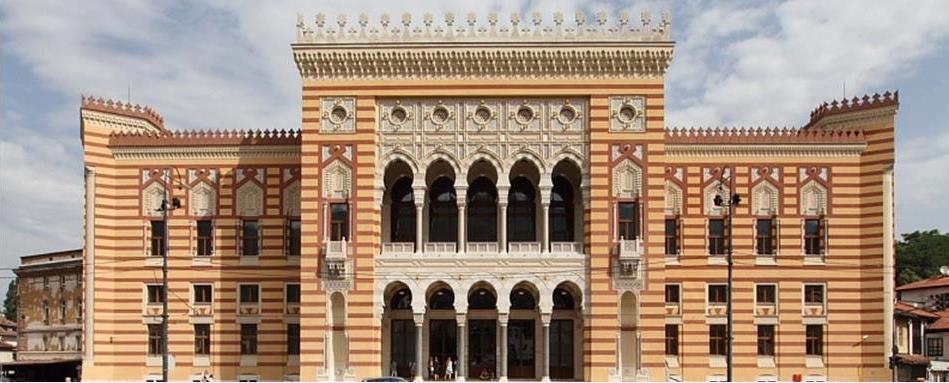
\includegraphics[scale =0.15]{orig.jpg}
   \hspace{0.2cm}
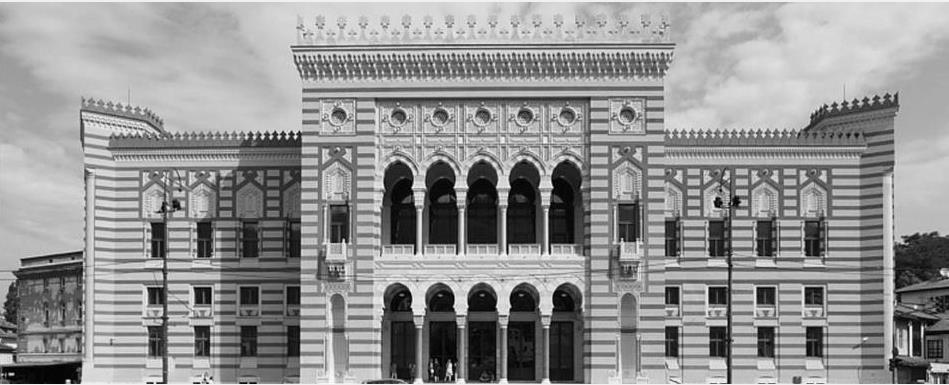
\includegraphics[scale =0.15]{gray.jpg}
}
\caption{Originalna slika i grayscale slika}
\label{fig}
\end{figure}
\begin{figure}[htbp]
\centerline{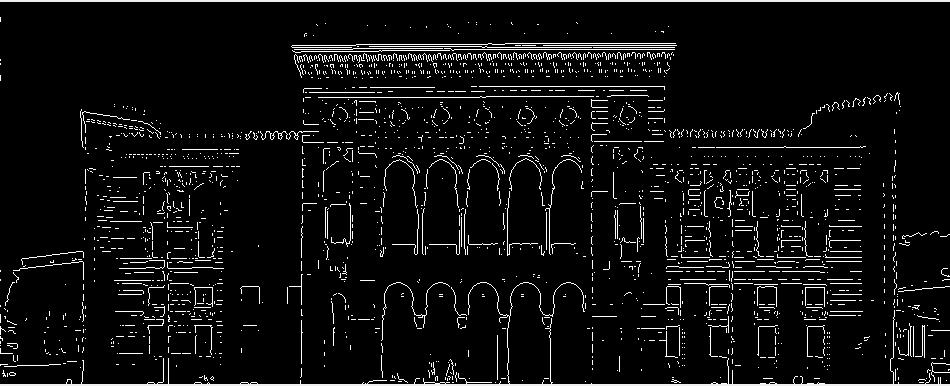
\includegraphics[scale =0.15]{matlabSobel.jpg}
   \hspace{0.2cm}
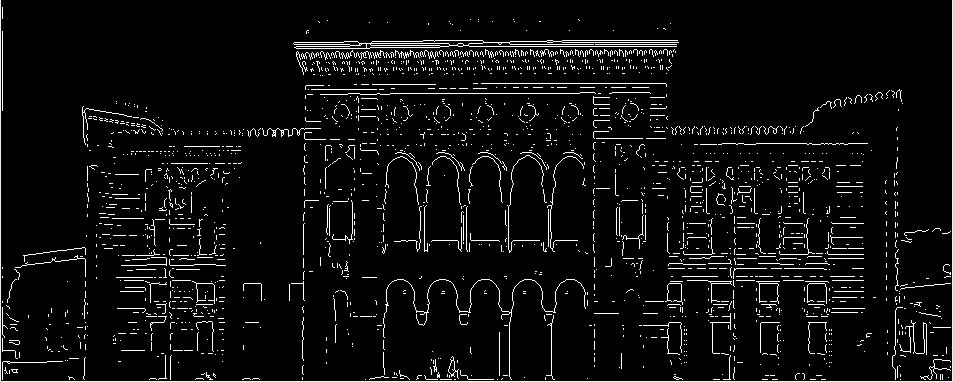
\includegraphics[scale =0.15]{sobelja.jpg}
}
\caption{Detektovane ivice pomoću ugrađene edge funkcije i implementirane SobelEdgeDetection funkcije}
\label{fig}
\end{figure}
\begin{figure}[h!]
\centerline{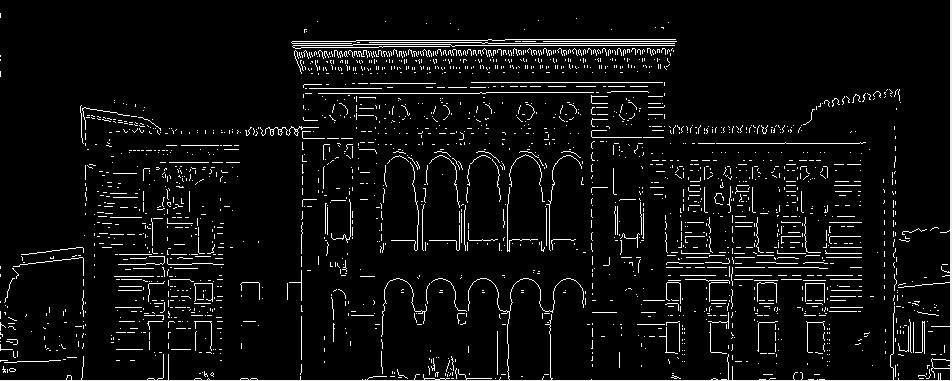
\includegraphics[scale =0.15]{matlabPrewit.jpg}
   \hspace{0.2cm}
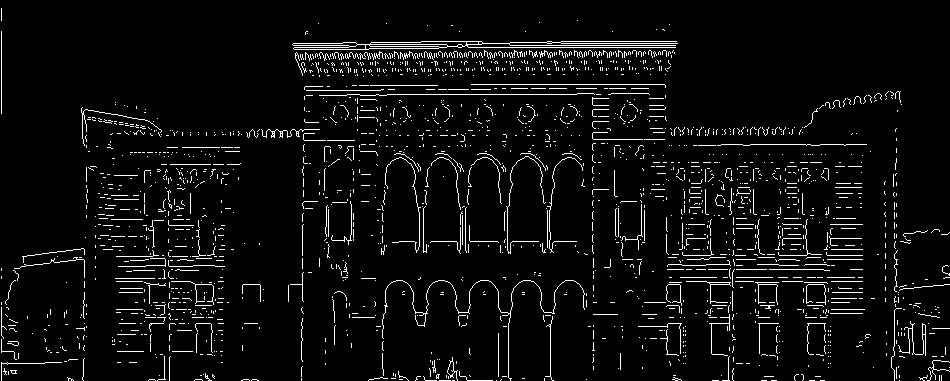
\includegraphics[scale =0.15]{japrewit.jpg}
}
\caption{Detektovane ivice pomoću ugrađene edge funkcije i implementirane PrewittEdgeDetection funkcije}
\label{fig}
\end{figure}
\begin{figure}[h!]
\centerline{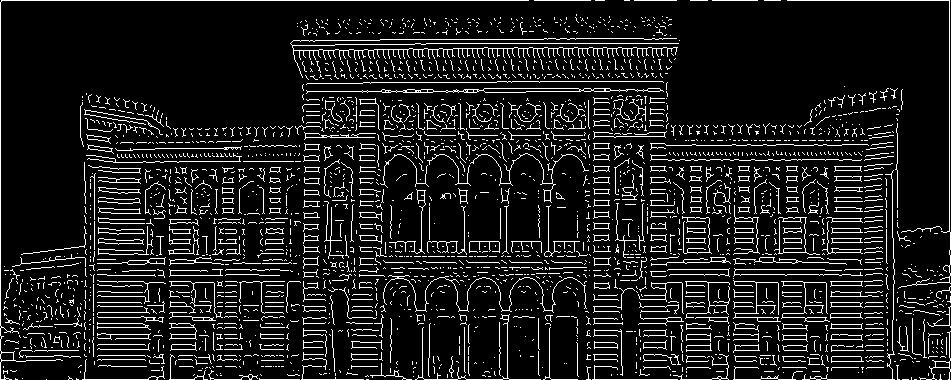
\includegraphics[scale =0.15]{matlablog.jpg}
   \hspace{0.2cm}
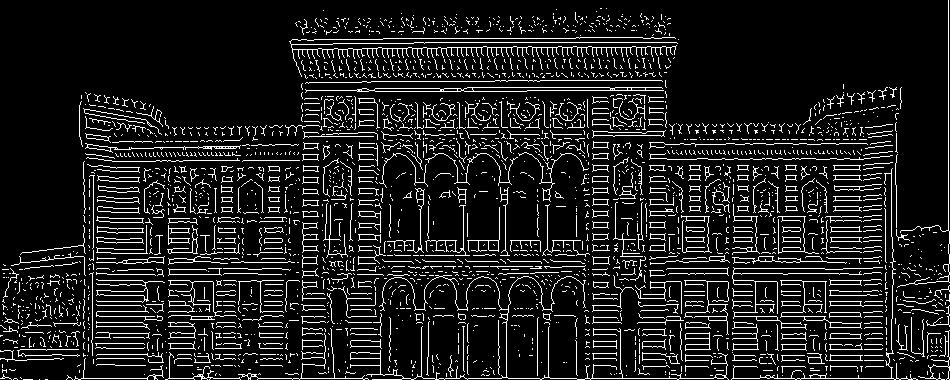
\includegraphics[scale =0.15]{jalog.jpg}
}
\caption{Detektovane ivice pomoću ugrađene edge funkcije i implementirane LogEdgeDetection funkcije}
\label{fig}
\end{figure}
\begin{figure}[h!]
\centerline{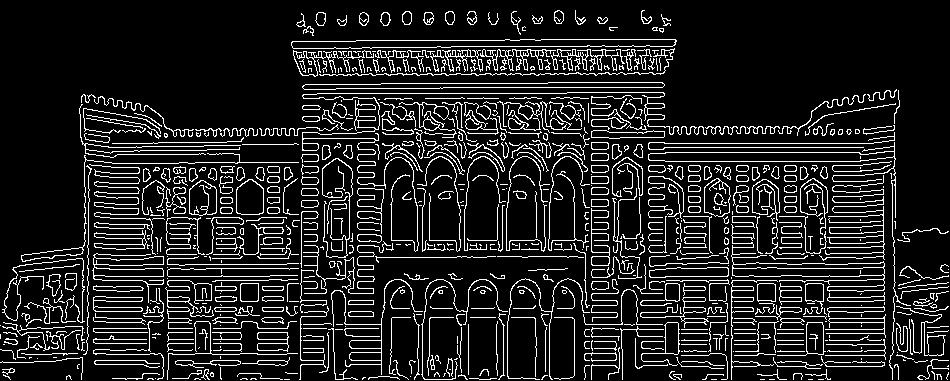
\includegraphics[scale =0.15]{cem.jpg}
   \hspace{0.2cm}
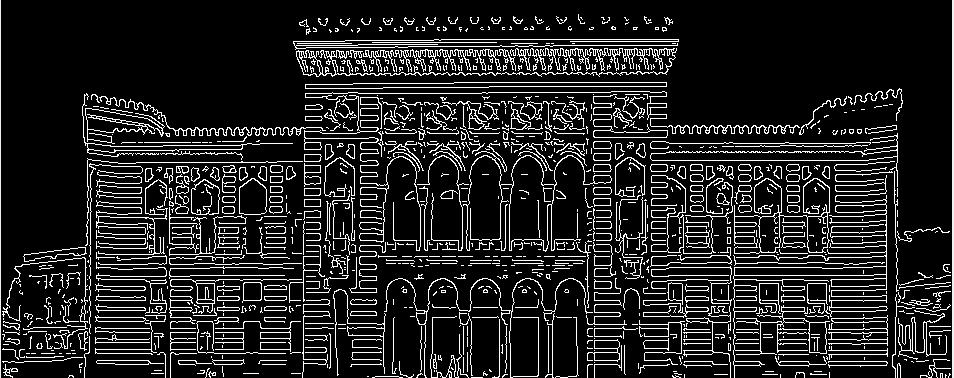
\includegraphics[scale =0.15]{ceja.jpg}
}
\caption{Detektovane ivice pomoću ugrađene edge funkcije i implementirane CannyEdgeDetection funkcije}
\label{fig}
\end{figure}
Na slikama 5, 6 i 7 su prikazani rezultati pozivanja ugrađenih i implementiranih funkcija za detekciju ivica. Za detekciju ivica Matlab ima ugrađenu funkciju \textit{edge} kojoj se proslijedi slika u grayscale formatu te parametar kojim se specificira koji algoritam će se primjeniti za dobijanje ivica. Također moguće je proslijedit i parametar praga(za Canny algoritam se proslijedi vektor $[T_{min},  T_{max}]$) i standardnu devijaciju ukoliko se koristi LoG algoritam. \\U tablici 1 su data vremena izvršavanja ugrađenih i implementiranih funkcija. Vremena su mjerena koristeći Matlab funkciju  \textit{timeit} koja više puta poziva funkciju čije vrijeme izvršavanja mjerimo i vraća srednju vrijednost. Funkcije su testirane na računaru čije su karakteristike: 
\begin{itemize}
    \item Procesor:  Intel(R) Core(TM) i5-3320M CPU @2.60Ghz 2.60Ghz,
    \item RAM: 4.00 GB,
    \item Operativni sistem: Windows 10.
\end{itemize} 

\begin{table}[h!]
\begin{center}
\caption{Vremena izvršavanja ugrađenih i implementiranih funkcija}
\begin{tabular}{|c|c|c|l}
\cline{1-3}
\multicolumn{3}{|c|}{\textbf{Vrijeme izvršavanja {[}s{]}}} &  \\ \cline{1-3}
Algoritam  & Ugrađena funkcija  & Implementirana funkcija  &  \\ \cline{1-3}
Sobel      & 0.0150             & 3.2293                   &  \\ \cline{1-3}
Prewitt    & 0.0138             & 3.6709                   &  \\ \cline{1-3}
LoG        & 0.0391             & 1.3567                   &  \\ \cline{1-3}
Canny      & 0.0355             &   0.7746                        &  \\ \cline{1-3}

\end{tabular}

\end{center}
\end{table}
\section{Zaključak}
Iz prikazanih rezultata se može zaključiti da ne postoji velika razlika u rezultatima koji su dobijeni korištenjem ugrađenih funkcija i rezultatima implemetiranih funkcija. Ako uporedimo rezultate koje su dali algoritmi zaključujemo da je Cannyev algoritam dao najbolji rezultat jer je isključio dosta 'slabih' ivica. Ovo nije bilo neočekivano jer je Cannyev algoritam i najkompleksniji. Bitno je napomenuti da je za implementirane funkcije potrebno mijenjati prag segmentacije za razliku od ugrađenih funkcija koje računaju prag koristeći Otsu algoritam. Kako je za bilo kakvu industrijsku primjenu važno automatizirati algoritam to je važno pronaći optimalne parametre što se može postići metodom pokušaja i greške. S aspekta vremena izvršavanja ugrađene funkcije se daleko brže izvršavaju u odnosu na implementirane.

\begin{thebibliography}{00}
\bibitem{b1} Gonzalez, R.C. and Woods, R.E., 2002. Digital image processing [M]. Publishing house of electronics industry, 141(7).
\bibitem{b2} Maini, R. and Aggarwal, H., 2008. Study and comparison of various image edge detection techniques. International journal of image processing (IJIP), 3(1).
\bibitem{b3} Sonka, M., Hlavac, V. and Boyle, R., 2014. Image processing, analysis, and machine vision. Cengage Learning.
\bibitem{b4} Canny, J., 1987. A computational approach to edge detection. In Readings in computer vision (pp. 184-203). Morgan Kaufmann.
\bibitem{b5} Zarei, A., 2017. Implementing Sobel and Canny Edge Detection Algorithms,University of Arizona. unpublished
\bibitem{b6} Gonzalez, R.C., Woods, R.E. and Eddins, S.L., 2009. Digital image processing using MATLAB. 2004. Publisher T. Robbins, Printed in USA, 11, pp.531-534.
\end{thebibliography}

\end{document}
